\documentclass[12pt,fleqn]{article}
\usepackage{
  amsmath,
  booktabs,
  geometry,
  graphicx,
  microtype,
  parskip,
}
\usepackage[shortlabels]{enumitem}

\geometry{margin=3cm}

% equation line spacing
\setlength{\jot}{0.5cm}

% meta data
\newcommand{\chapter}{Project Part 1 \-- Data and Descriptive Statistics}
\newcommand{\authorname}{Amo DelBello}
\newcommand{\classdescription}{MATH 1350-D2}
\newcommand{\classname}{Introduction to Statistics, Fall 2022}
\newcommand{\assignment}{Demonstrate: \chapter}

\newcommand{\problem}[1]{\vspace{5ex}\section*{\chapter-#1}}
\newcommand{\thead}[1]{\textnormal{\textbf{#1}}}
\newcommand{\tvspace}{\vspace{.25cm}}

\title{\classdescription\ \\ \classname\ \\ $\ $ \\ \assignment}
\author{\authorname}
\date{\today}


\begin{document}

\maketitle

For this project I chose the \textbf{NutritionDataFastFood2017.xlsx} as the source of data.

\section{Understand How and Why the Data was Collected}
\begin{enumerate}
\item \textbf{What is your best guess about the sampling methodology?}

  I believe it likely that the data for this study comes from the individual restaurants themselves, or from third parties hired by the restaurants. The fine print on the McDonalds website states:
  \begin{quote}
    \begin{footnotesize}
    ``The nutrition information on this website is derived from testing conducted in accredited laboratories, published resources, or from information provided from McDonald's suppliers.''
    \end{footnotesize}
  \end{quote}
  It's likely the other restaurants in the study follow similar methods. It's unclear what the sampling methodology is, e.g.~simple random, stratified, convenience, etc, and how it might vary from one restaurant to another. One would hope that the process is sufficiently regulated by the appropriate government agency (FDA) and that the data here is accurate and a good representation of the populations from which the samples were taken.

\item \textbf{What was the purpose of the study?}

  The purpose of the study appears to be the comparison of various macronutrients contained in fast food menu items.

\pagebreak
\item \textbf{What do each of the elements mean?}

  The only source of data provided is a spreadsheet listing various fast food menu items, their origin, i.e.\ respective fast food restaurant, and several macronutrient values associated with each item. The fields are as follows:
  \begin{itemize}
  \item Fast Food Restaurant
  \item Item Type
  \item Serving Size (g)
  \item Calories
  \item Total Fat (g)
  \item Saturated Fat (g)
  \item Trans Fat (g)
  \item Sodium (mg),
  \item Carbs (g),
  \item Sugars (g),
  \item Protein (g)
  \end{itemize}
\end{enumerate}

\section{Describe the Characteristics of the Data Set}
Using this data I will attempt to determine if we can distinguish whether or not specific fast food restaurants are ``healthier'' than others.

I am choosing to focus on a single macronutrient --- calories. If successful, the same methods could be used with the other fields as well. In an attempt to compare ``apples to apples'', so to speak, I will calculate each item's \textit{per gram} calorie value and use that for any further calculations.

We will use the standard deviation of all menu items as a baseline from which to compare that of the specific restaurants. The measures of center and standard deviation of the newly calculated ``calories per gram'' field taking all 123 menu items into account are:

  \vspace{.25cm}
  \begin{tabular}{@{}ll@{}}
    \thead{Measures of Center (cal/g)} & \\
    \toprule
    Mean & 2.505 \\
    Median & 2.5 \\
    Range & 2.908 \\
    Midrange & 2.676 \\
  \end{tabular}

  \begin{tabular}{@{}ll@{}}
    \textbf{Standard Deviation} & 0.527 \\
  \end{tabular}
  \vspace{.25cm}

When we group this data by restaurant we are able to see how each differs from the baseline:

  \vspace{.25cm}
  \begin{tabular}{@{}lllllll@{}}
    \thead{Restaurant} & \thead{Mean} & \thead{Num Items} & \thead{Std. dev.} & \thead{+/- SD} & \thead{Median} & \thead{Range}  \\
  \toprule
  Hardee's	    & 2.40725	& 12	& 0.288 & -0.239        & 2.435	 & 1.069 \\
  Dairy Queen	    & 2.5553	& 10	& 0.338 & -0.189	& 2.5585 & 1.225 \\
  Jack in the Box & 2.84225	& 12	& 0.359 & -0.168	& 2.9895 & 1.135 \\
  McDonald's	    & 2.5103636	& 11	& 0.364 & -0.163	& 2.566	 & 1.317 \\
  Carl's Jr.	    & 2.3814615	& 13	& 0.372 & -0.155	& 2.382	 & 1.237 \\
  Burger King	    & 2.5046364	& 11	& 0.398 & -0.129	& 2.5	 & 1.402 \\
  Wendy's	    & 2.5756364	& 11	& 0.478 & -0.049	& 2.566	 & 1.584 \\
  Sonic	    & 2.644	& 11	& 0.553 & 0.026	& 2.92	 & 1.602 \\
  Whataburger	    & 2.211	& 12	& 0.616 & 0.089	& 2.0485 & 2.04  \\
  In-N-Out Burger & 2.0848	& 5	& 0.620 & 0.093	& 1.838	 & 1.555 \\
  Chick-fil-A	    & 2.1452	& 5	& 0.808 & 0.281	& 2.281	 & 1.954 \\
  White Castle    & 2.83	& 10	& 0.862 & 0.335	& 2.9185 & 2.908 \\
  \bottomrule
\end{tabular}
\vspace{.25cm}

A summary graph also shows the differences between each restaurant:
\begin{figure}[ht]
  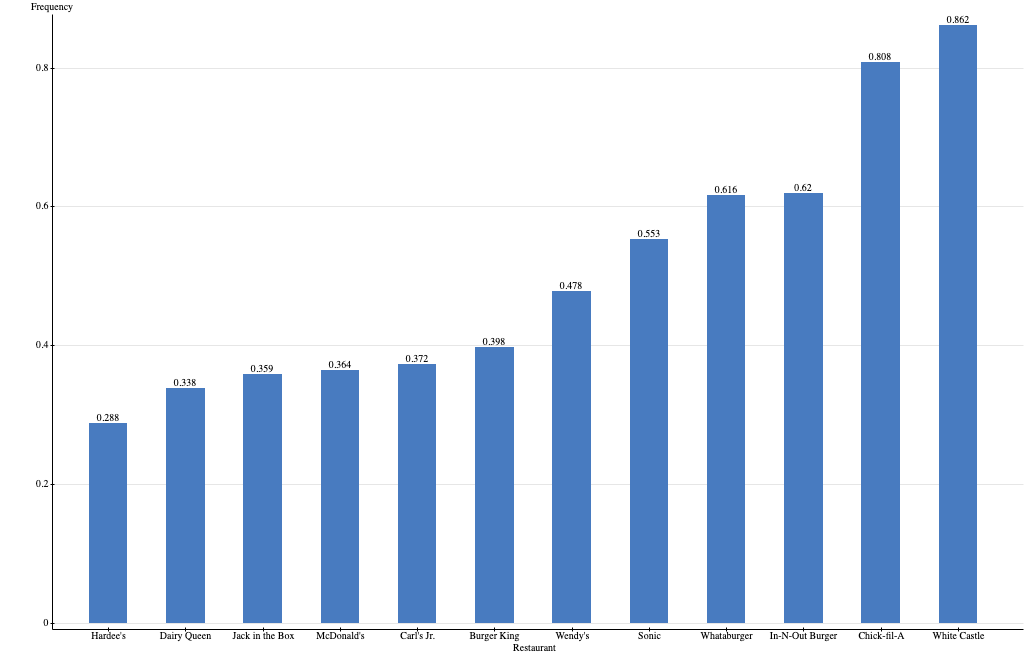
\includegraphics[width=6in]{assets/std-dev-restaurants.png}
  \caption{Standard Deviation of Calories per gram of food}
\end{figure}

\pagebreak
We can see that there are no significantly low or high values in the data. However it is clear that some restaurants have a lower calorie count per gram than others.

As fast food, in general, consists of high calorie ingredients with low nutritional content, it's best to limit one's consumption, or avoid altogether. If one \textit{must} consume fast food, analysis of the data confirms the following, with respect to calorie content:

\textbf{The healthiest choices, among the restaurants in the study are Hardees, Dairy Queen, and Jack in the Box. The unhealthiest are White Castle, Chick-fil-A, and In-N-Out-Burger.}

It would be interesting to see whether these findings mirror the same with respect to sugar, carbohydrates, and other macronutrients.

\end{document}
%%% Local Variables:
%%% mode: latex
%%% TeX-master: t
%%% End:
